\documentclass[a4paper,12pt]{article}
%%%%%%%%%%%%%%%%%%%%%%%%%%%%%%%%%%%%%%%%%%%%%%%%%%%%%%%%%%%%%%%%%%%%%%%%%%%%%%%%%%%%%%%%%%%%%%%%%%%%%%%%%%%%%%%%%%%%%%%%%%%%%%%%%%%%%%%%%%%%%%%%%%%%%%%%%%%%%%%%%%%%%%%%%%%%%%%%%%%%%%%%%%%%%%%%%%%%%%%%%%%%%%%%%%%%%%%%%%%%%%%%%%%%%%%%%%%%%%%%%%%%%%%%%%%%
\usepackage{eurosym}
\usepackage{vmargin}
\usepackage{amsmath}
\usepackage{graphics}
\usepackage{epsfig}
\usepackage{subfigure}
\usepackage{fancyhdr}

\setcounter{MaxMatrixCols}{10}
%TCIDATA{OutputFilter=LATEX.DLL}
%TCIDATA{Version=5.00.0.2570}
%TCIDATA{<META NAME="SaveForMode"CONTENT="1">}
%TCIDATA{LastRevised=Wednesday, February 23, 201113:24:34}
%TCIDATA{<META NAME="GraphicsSave" CONTENT="32">}
%TCIDATA{Language=American English}

\pagestyle{fancy}
\setmarginsrb{20mm}{0mm}{20mm}{25mm}{12mm}{11mm}{0mm}{11mm}
\lhead{MA4128} \rhead{Kevin O'Brien} \chead{Cluster Analysis  } %\input{tcilatex}

\begin{document}


\section{The Two-Step Cluster Analysis}
The Two-Step Cluster Analysis is an exploratory tool designed to reveal natural groupings (or clusters) within a data set that would otherwise not be apparent. The algorithm employed by this procedure has several desirable features that differentiate it from traditional clustering techniques:

\begin{itemize}
	\item \textbf{\textit{Handling of categorical and continuous variables:}} By assuming variables to be independent, a joint \textbf{\textit{multinomial-normal distribution}} can be placed on categorical and continuous variables. (Interesting, but not examinable).
	
	\item \textbf{\textit{Automatic selection of number of clusters:}} By comparing the values of a \textbf{\textit{model-choice criterion}} across different clustering solutions, the procedure can automatically determine the optimal number of clusters.
	
	\item \textbf{\textit{Scalability:}} By constructing a \textbf{\textit{cluster features}} (CF) tree that summarizes the records, the Two-Step algorithm allows you to analyze large data files.\\ The Two-Step Cluster Analysis requires only one pass of data, which is computationally efficient, important for very large data files.
	
\end{itemize}


\section{Two-Step Cluster Analysis}
\begin{itemize}
	\item 
	
	When you have a really large data set or you need a clustering procedure that can rapidly form clusters on the basis of either categorical or continuous data, neither of the two main types of procedures are entirely appropriate. Hierarchical clustering requires a matrix of distances between all pairs of cases, and k-means requires shuffling cases in and out of clusters and knowing the number of clusters in advance.
	
	\item The Two-Step Cluster Analysis procedure was designed for such applications. The name two-step clustering is already an indication that the algorithm is based on a two-stage approach
	\begin{itemize}
		\item[$\ast$] In the first stage, the algorithm undertakes a procedure that is very similar to the k-means algorithm. \\Based on these results, the two-step
		procedure conducts a modified hierarchical agglomerative clustering procedure that
		combines the objects sequentially to form homogenous clusters.

		
\end{itemize}
\end{itemize}
	\subsection{Step 1: Preclustering: Making Little Clusters}
	\begin{itemize}
		\item The first step of the two-step procedure is formation of preclusters. The goal of
		preclustering is to reduce the size of the matrix that contains distances between all
		possible pairs of cases.    \item Preclusters are just clusters of the original cases that are used
		in place of the raw data in the hierarchical clustering.     \item As a case is read, the algorithm
		decides, based on a distance measure, if the current case should be merged with a
		previously formed precluster or start a new precluster. When preclustering is complete,
		all cases in the same precluster are treated as a single entity.     \item The size of the distance
		matrix is no longer dependent on the number of cases but on the number of preclusters.
	\end{itemize}
	\subsection{Step 2:	Hierarchical Clustering}
\begin{itemize}
\item In the second step, SPSS uses the standard hierarchical clustering algorithm on the
preclusters. Forming clusters hierarchically lets you explore a range of solutions with
different numbers of clusters.
\\ \textit{Tip: The Options dialog box lets you control the number of preclusters. Large numbers
	of preclusters give better results because the cases are more similar in a precluster;
	however, forming many preclusters slows the algorithm}.


\end{itemize}



\section{Pre-Clustering}
\begin{itemize}
	\item In two-step clustering, to make large problems tractable, in the first step, cases are
	assigned to \textbf{\textit{preclusters}}. 
	\item In the second step, the preclusters are clustered using the
	hierarchical clustering algorithm. \begin{itemize}
		\item[$\ast$] You can specify the number of clusters you want or
	let the algorithm decide based on preselected criteria.
	\end{itemize}
	\item In general, the larger the number of sub-clusters produced by the pre-cluster step, the more accurate the final result is. However, too many sub-clusters will slow down the clustering during the second step.
	
	\item The maximum number of sub-clusters should be carefully chosen so that it is large enough to produce accurate results and small enough not to slow down the second step clustering.
	
\end{itemize}



\section{Important Considerations for Two-Step Clustering}
\subsection{Cluster Features Tree}

\begin{itemize}
	\item Two-Step Cluster Analysis is done by building a so-called \textbf{\textit{cluster feature tree}} whose \textbf{\textit{leaves}} represent distinct objects in the dataset. 
	\item The procedure can handle categorical and continuous variables simultaneously and offers the user the flexibility to specify the cluster numbers as well as the maximum number of clusters, or to allow the technique to automatically choose the number of clusters on the basis of statistical evaluation criteria.
	
	\item Additionally, the procedure indicates each variable’s importance for the construction of a specific cluster. These desirable features make the somewhat less popular two-step clustering a viable alternative to the traditional
	methods.
	
	
\end{itemize}


\subsection{Types of Data} The Two-Step procedure works with both continuous and categorical variables. Cases represent objects to be clustered, and the variables represent attributes upon which the clustering is based.



\subsection{Case Order}
\begin{itemize}
    \item Note that the cluster features tree and the final solution may depend on the order of objects (or cases). To minimize order effects, randomly order the cases. 
    \item It is recommended to obtain several different solutions with cases sorted in different random orders to verify the stability of a given solution. 
    \item In situations where this is difficult due to extremely large file sizes, multiple runs with a sample of cases sorted in different random orders might be substituted.
\end{itemize}



\section{SPSS Implementation}

\begin{itemize}
\item To implement a Two-Step Cluster Analysis in SPSS, you use the following options:\\
\textbf{\textit{Analyze $>$ Classify $>$ TwoStep Cluster}}.

\item \textbf{Distance Measure} Log likelihood distance measures are the default; Euclidean distance can be used if all variables are continuous. (Log likelihood distance measures are not part of course).

\item \textbf{Count of Continuous Variables} Continuous variables are standardized by default. The variables
are standardized so that they all contribute equally to the distance or similarity between cases.

\item \textbf{Number of clusters} You can specify the number of clusters, or you can let the algorithm select
the optimal number based on either the Schwarz Bayesian criterion (BIC) or the Akaike
information criterion (AIC).

\item \textbf{Clustering Criterion} BIC and AIC are offered with the default being BIC.
\end{itemize}



\section{Graphical Outputs}
\begin{itemize}
    \item 
The lower part of the output  indicates the quality of the cluster
solution. The silhouette measure of cohesion and separation is a measure of the
clustering solution’s overall goodness-of-fit. 
\item It is essentially based on the average
distances between the objects and can vary between -1 and +1. Specifically, a
silhouette measure of less than 0.20 indicates a poor solution quality, a measure
between 0.20 and 0.50 a fair solution, whereas values of more than 0.50 indicate a
good solution. 
\item In our case, the measure indicates a satisfactory (``fair") cluster quality. Consequently, you can
proceed with the analysis by double-clicking on the output. This will open up the
model viewer, an evaluation tool that graphically presents the structure
of the revealed clusters.
\item 

The model viewer provides us with two windows: the main view, which initially
shows a model summary (left-hand side), and an auxiliary view, which initially
features the cluster sizes (right-hand side).
\item At the bottom of each window, you can
request different information, such as an overview of the cluster structure and the
overall variable importance.
\end{itemize}
\begin{figure}
\centering
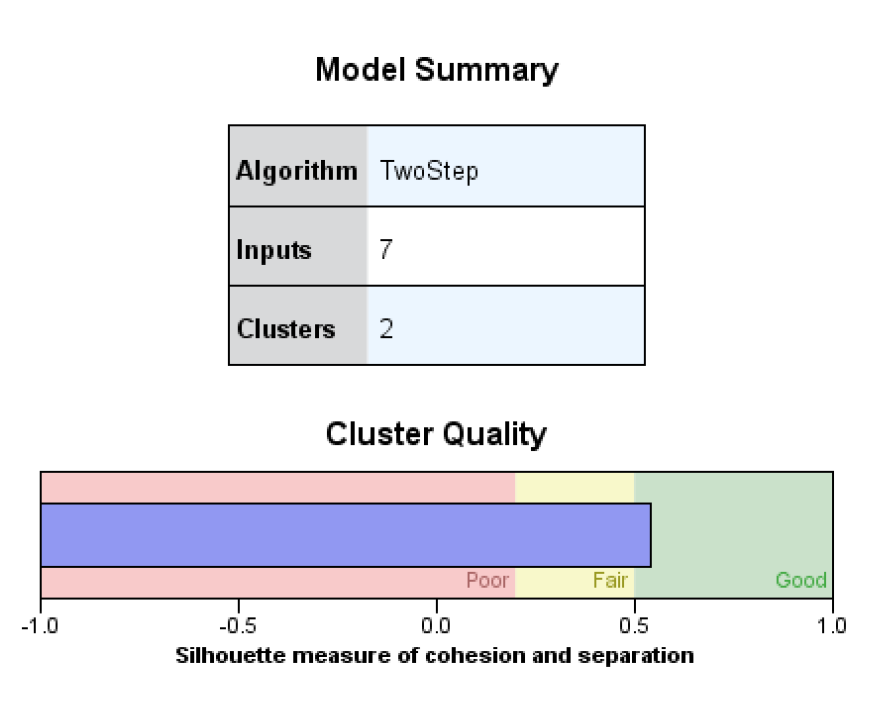
\includegraphics[width=0.7\linewidth]{images/silhouette}
\caption{}
\label{fig:silhouette}
\end{figure}

%%%%%%%%%%%%%%%%%%%%%%%%%%%%%%%%%%%%%%%%%%%%%%%%%%%%%%%%%%%

\section*{Settings}
Some of the options you can specify when using two-step clustering are:

\begin{itemize}
	\item \textbf{Standardization:} The algorithm will automatically standardize all of the variables
	unless you override this option.
	\item \textbf{Distance measures:} If your data are a mixture of continuous and categorical variables,
	you can use only the log-likelihood criterion. The distance between two clusters
	depends on the decrease in the log-likelihood when they are combined into a single
	cluster. If the data are only continuous variables, you can use the Euclidean
	distance between two cluster centers. Depending on the distance measure selected,
	cases are assigned to the cluster that leads to the largest log-likelihood or to the cluster
	that has the smallest Euclidean distance.
	
	
\item \textbf{Number of clusters:} You can specify the number of clusters to be formed, or you can let
	the algorithm select the optimal number based on either the Schwarz Bayesian
	Criterion or the Akaike information criterion.
	
	
\item \textbf{Outlier handling:} You have the option to create a separate cluster for cases that don't fit
	well into any other cluster.
	\item 
	\textbf{Range of solutions:} You can specify the range of cluster solutions that you want to see.
\end{itemize}




\section{Measures of Fit}
\begin{itemize}
	\item Two-Step Cluster Analysis guides the decision of how many clusters to retain from the data by
	calculating measures-of-fit such as \textbf{\textit{Akaike’s Information Criterion (AIC)}} or \textbf{\textit{Bayes Information Criterion (BIC)}}.
	
	\item These are relative measures of goodness-of-fit and are used to compare different
	solutions with different numbers of segments.(``Relative" means that these criteria
	are not scaled on a range of, for example, 0 to 1 but can generally take any value.)
	Compared to an alternative solution with a different number of segments, smaller
	values in AIC or BIC indicate an increased fit.
	
\item SPSS computes solutions for different segment numbers (up to the maximum number of segments specified before) and
chooses the appropriate solution by looking for the smallest value in the chosen
criterion. However, which criterion should we choose?
\begin{itemize}
	\item[$\ast$] AIC is well-known for
	overestimating the correct number of segments
	\item[$\ast$] BIC has a slight tendency
	to underestimate this number.
\end{itemize}

	
	\item Thus, it is worthwhile comparing the clustering
	outcomes of both criteria and selecting a smaller number of segments than
	actually indicated by AIC. Nevertheless, when running two separate analyses,
	one based on AIC and the other based on BIC, SPSS usually renders the same
	results. 
\end{itemize}





\subsection{AIC and BIC in Two-Step Cluster Analysis}

\begin{itemize}
	\item Once you make some choices or do nothing and go with the defaults, the clusters are
	formed. At this point, you can consider whether the number of clusters is ``good". If
	automated cluster selection is used, SPSS prints a table of statistics for different
	numbers of clusters, an excerpt of which is shown in the figure below.
	\item  You are interested
	in finding the number of clusters at which the Schwarz BIC becomes small , but also the change in BIC between
	adjacent number of clusters is small. 
	
	\item The decision of how much benefit accrued by another cluster is very subjective. In addition to the BIC, a high ratio of distance of measures is desirable. In the figure below, the number of clusters with this highest ratio is three.
	
	\begin{figure}[h!]
		\begin{centering}
			% Requires \usepackage{graphicx}
			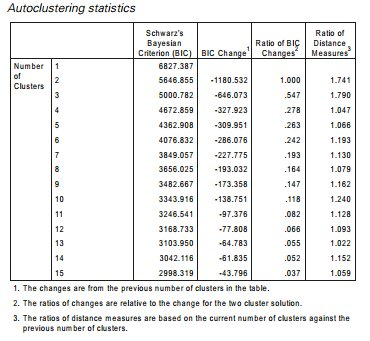
\includegraphics[width=14.5cm]{images/TwoStep1.jpg}\\
			\caption{Schwarz Bayesian Information Criterion}
		\end{centering}
	\end{figure}
\end{itemize}














\end{document}

\section*{Standby: Akaike Information Criterion}

Information Criterions
We define two types of information criterion: the Akaike Information Criterion (AIC) and the
Schwarz?s Bayesian Information Criterion (BIC). The Akaike information criterion is a measure
of the relative goodness of fit of a statistical model.
AIC = 2p ? 2 ln(L)


%=================================================%
\begin{itemize}
	\item p is the number of predictor variables in the model.
	\item L is the value of the Likelihood function for the model in question.
	\item For AIC to be optimal, n must be large compared to p.
\end{itemize}

An alternative to the AIC is the Schwarz BIC, which additionally takes into account the
sample size n.
BIC = p ln n ? 2 ln(L)
When using the AIC (or BIC) for selecting the optimal model, we choose the model for which
the AIC (or BIC) value is lowest.



\begin{itemize}
	\item Akaike?s information criterionis a measure of the goodness of fit of an estimated statistical
	model. The AIC was developed by Hirotsugu Akaike under the name of ?an information
	criterion? in 1971.
	\item The AIC is a model selection tool i.e. a method of comparing two or more candidate
	regression models. The AIC methodology attempts to find the model that best explains
	the data with a minimum of parameters. (i.e. in keeping with the law of parsimony)
	\item The AIC is calculated using the ?likelihood function? and the number of parameters .
	The likelihood value is generally given in code output, as a complement to the AIC.
	(Likelihood function is not on our course)
	\item Given a data set, several competing models may be ranked according to their AIC, with
	the one having the lowest AIC being the best. (Although, a difference in AIC values of
	less than two is considered negligible).
	
\end{itemize}

%------------------------------------------------------------------------------%\end{document}
